
\renewcommand\refname{Literaturverzeichnis}
\printbibliography
\cleardoublepage
\listoffigures


\clearpage

\section{Anhang}
    \subsection{Aufgabenstellung}
        \begin{figure}[h]
            \centering
            \begin{minipage}[b]{0.8\textwidth}
                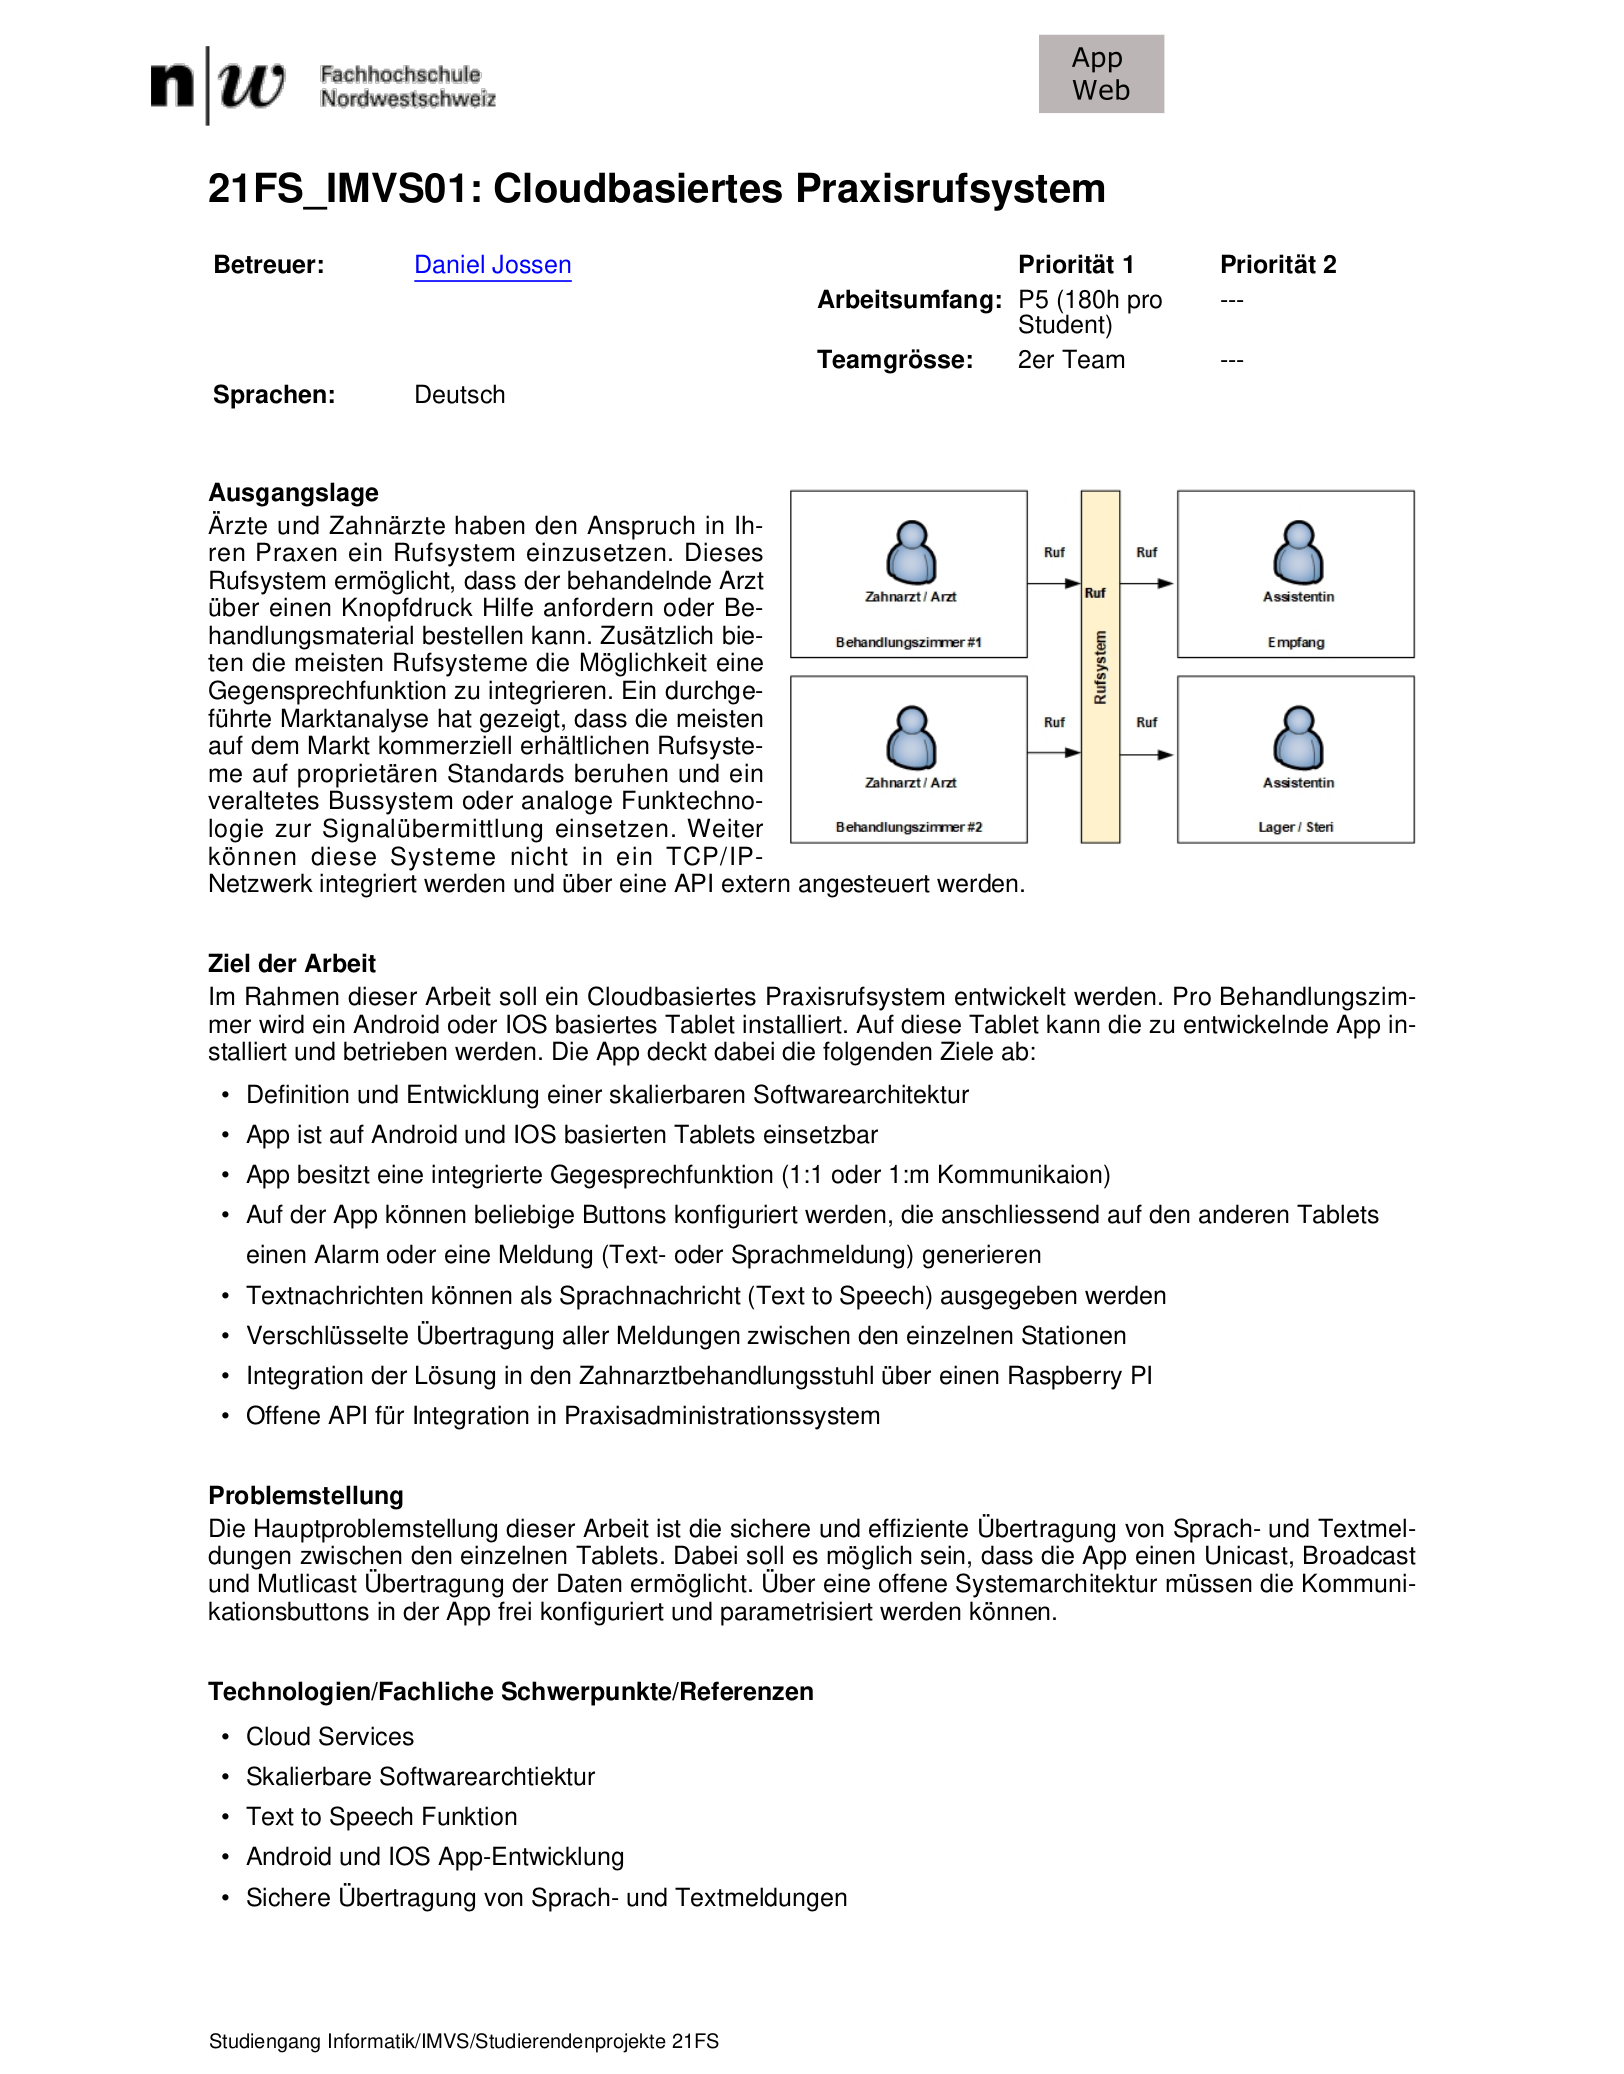
\includegraphics[width=\textwidth]{graphics/aufgabenstellung}
                \caption{Aufgabenstellung}
            \end{minipage}
        \end{figure}

    \subsection{Quellcodeverwaltung}

    Sämtlicher Quellcode der im Rahmen des Projektes entsteht, wurde mit Git verwaltet. Der Quellcode ist für Berechtigte unter dem Projekt IP5-Cloudbasiertes-Praxisrufsystem auf github.com einsehbar.
    (Referenz https://github.com/IP5-Cloudbasiertes-Praxisrufsystem). Berechtigungen können bei Joshua Villing oder Kevin Zellweger angefordert werden.

    \begin{itemize}
        \item IP5-praxis-mobile-client
        \item IP5-praxis-cloud-service
        \item IP5-praxis-admin-ui
        \item IP5-praxis-documentation
    \end{itemize}

    \subsection{Benutzerhandbuch}
    \subsection{Betriebshandbuch}
    \subsection{Entwicklerdokumentation}
    \subsection{Ehrlichkeitserklärung}
